\chapter{Evaluation}
\chlab{evaluation}

In order to determine which of the two implementations of \oframp{} is better in which aspect, and to evaluate the project in general, the system will be subjected to a user study~(see also \chref{approach}). This chapter will discuss what we will evaluate in the user studies in more detail. We describe the tasks the participants have to complete~(\secref{ev_tasks}), the questionnaires they have to fill in~(\secref{ev_questionnaires}), and how to calculate certain scores and what their meaning should be~(\secref{ev_analysis}).

The full set of experiment instructions, as was sent to the users, is provided in \appref{instructions}. This does not include the invitation email, or accompanying text, but rather just the set of tasks. Additionally, all questionnaires that participants were asked to complete can be found in \appref{questionnaires}.



\section{User tasks}
\seclab{ev_tasks}
As discussed in \secref{ra_studies}, the participants of the user studies will be equally divided over two groups, each of which will be instructed to use both versions of the system in a different order. The experiment participants will be asked to complete the Demo mode first, such that they can get used to the system, and get some instructions on how to use it. Next, they will be asked to parameterise a small, simple molecule, followed by a larger, more complex one. By starting with a small molecule, it should be easier to learn how to use the tool, and users should not be scared by the magnitude of their first task. The larger molecule they have to parameterise later, on the other hand, will be a better reflection of the actual use of the system.

After completely parameterising the two molecule, users are asked to fill in a short questionnaire about the version of the system they used~(see \secref{ev_questionnaires}), after which they are asked to switch to the other version of \oframp. They then have to complete the same tasks, including following the demo, for two additional molecules. Again, this will be a small and a large molecule, and participants will be asked to complete a similar questionnaire. When all this has been done, a final questionnaire about \oframp{} in general needs to be filled in. By that time, users are completely done, and will have spent around an hour in total~(see \secref{ra_studies}).

\begin{figure}[h!]
\centering
\begin{subfigure}[t]{0.48\textwidth}
\centering
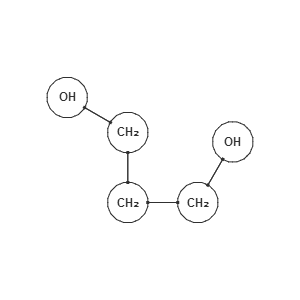
\includegraphics[width=\textwidth]{img/10321.png}
\caption{1,3-propandiol (PDO), \texttt{ATB ID} 10321.}
\figlab{10321}
\end{subfigure}%
~
\begin{subfigure}[t]{0.48\textwidth}
\centering
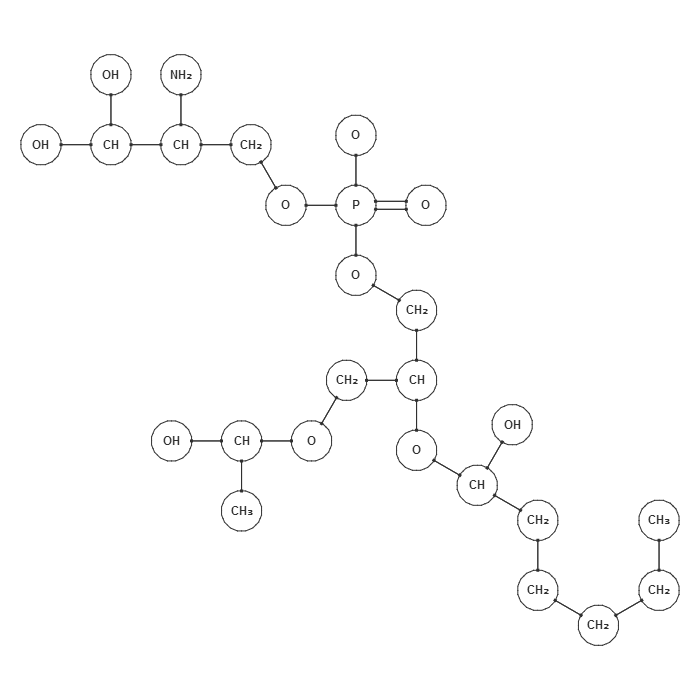
\includegraphics[width=\textwidth]{img/16978.png}
\caption{\_V3M, \texttt{ATB ID} 16978.}
\figlab{16978}
\end{subfigure}%
\\[1em]
\begin{subfigure}[t]{0.48\textwidth}
\centering
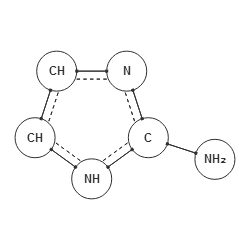
\includegraphics[width=\textwidth]{img/13913.png}
\caption{1h-imidazol-2-amine (2AI), \texttt{ATB ID} 13913.}
\figlab{13913}
\end{subfigure}%
~
\begin{subfigure}[t]{0.48\textwidth}
\centering
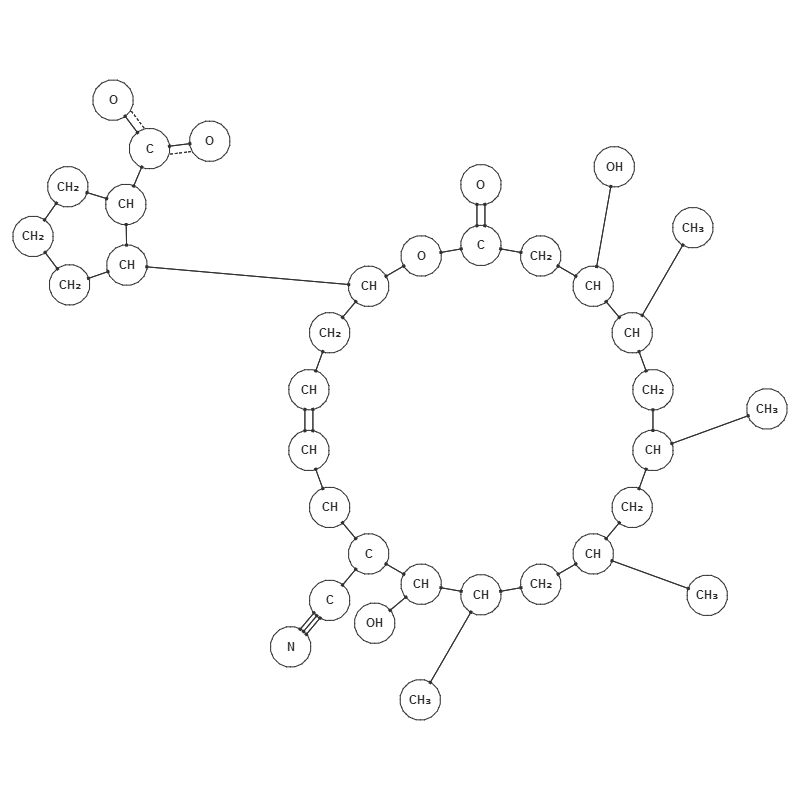
\includegraphics[width=\textwidth]{img/17738.png}
\caption{borrelidin (\_VOQ), \texttt{ATB ID} 17738.}
\figlab{17738}
\end{subfigure}
\caption{\oframp\ visualisations of the four molecules that are used in the user study.}
\figlab{ev_molecules}
\end{figure}

\Figref{ev_molecules} shows the molecules that participants have to parameterise in the experiment. Both participant groups will use these molecules in the same order, which is the order in which they are shown in the figure. We have selected them based on their size, and the fact that it is possible to fully parameterise them using the fragment repository of \oframp. In addition, we tried to choose different types of molecules, to see if the system works for all of them.

In order to make sure users are not prejudiced by the names of the two versions of the system, these names are never used in the instructions. In the final questionnaire they are simply referred to as 1 and 2, reflecting the first and second used version. The only other location where the difference can be observed is in the URLs to the two versions. Where the \IDa\ version has a URL ending in \verb|/n|, the \IDb\ version of the system can be accessed via \verb|/s|\footnote{The versions were initially called naive and smart respectively, hence the URLs.}. As the words `\IDa' and `\IDb' are never mentioned, users will not be able to infer the meanings of the characters. Furthermore, as they are not called `a' and `b', for instance, they will not be able to guess which version has been hypothesized to be the better one.

An extensive logging mechanism has been built into \oframp\footnote{This mechanism is only present in the special `experiment' version.}, that allows for easy usage statistics acquisition. It tries to record as much as it can; from browser details to system load times, and from mouse clicks to button presses. Every log message contains a time-stamp, such that the time difference between two log events can be calculated. They also include a message type, such that they can easily be filtered and counted. Finally, the resulting parameterisation is stored in the log as well, in order to be able to grade the user's performance~(see \secref{ev_analysis}).



\section{Questionnaires}
\seclab{ev_questionnaires}
The questions that users will be asked to answer after completing their tasks on either of the two versions of the system will mainly be questions about how they like the design and if they can see themselves using it. Additionally, they will be asked for suggestions on things that can be improved or added. This way, the user's experiences can be used to improve the system further, and to make it into something they really like to use.

The first half of this questionnaire will be based on the positive \verb|SUS| and \verb|UMUX-LITE| usability metrics~\cite{lewis2013umux}~(see also \secref{user_studies}). It will consist of the, for this tool, relevant questions from those metrics, followed by some questions about what they liked and disliked about the tool. To be certain that the questions are answered from the interaction design point of view, they will be asked from both the chemistry and interaction design perspectives. This gives the test subjects a place to put their comments on the chemical correctness, such that their feedback on the interaction design will truly concern the design.

After testing both the \IDa\ and \IDb\ versions of \oframp, and assessing them with the previously discussed questionnaires, a few more, general questions will be asked. These questions will concern what version the users liked best and why, if they want to see any functionality added to the system, and leave some room for additional comments. This will probably not provide new insights as to which version is liked better, as that can be inferred from the ratings obtained by the previous questionnaires. However, the answers to these questions will hopefully be able to help in the further development of \oframp.

The questionnaires, just like the experiment, needed to be conducted online. Because of this, they have been implemented as web forms using (a minor extension of) the questionnaire language \verb|QL|~\cite{erdweg2013state}. This allowed for easy definition of the form, without having to worry about validation or layout.



\section{Analysis}
\seclab{ev_analysis}
The results from the log of the user studies, combined with those obtained with the questionnaire, should be able to give an answer on which of the two interaction designs is preferable in which aspect. The version that gives good results in a short amount of time, and is also positively graded in the questionnaire, will be the overall better one. Furthermore, the timing and scoring results from the experiment alone will be able to answer the question if it is possible to do fragment-based molecule parameterisation at all. At least for one of the two versions both time consumption and parameterisation results should be reasonable.

In order to rate the user's parameterisation, the molecules that the user will be asked to parameterise should already have been parameterised using the conventional quantum mechanical calculations, and present in the ATB. This way, the user's results can be compared to the outcomes of the calculations, in order to establish a rating. The smaller the difference between the two, the better the performance of the user will be graded.

There are two different ways of calculating the user's result rating:
\begin{align*}
R &= |\Phi - C| & r &= \sum_{i = 1}^{n} |\delta_{i}|,
\end{align*}
\vspace{-1em}
\begin{align*}
\text{where} \quad \Phi &= \text{ATB total molecule charge},\\
C &= \text{\oframp{} total molecule charge},\\
n &= \text{total number of atoms in the molecule},\\
\delta_{i} &= \phi_{i} - c_{i},\\
\phi_{i} &= \text{ATB charge of the atom with index}~i,\\
c_{i} &= \text{\oframp{} charge of the atom with index}~i.
\end{align*}

First, it is interesting to know the difference in the total charge of the molecules, which is given by $R$. This is something that can be observed and minimised by the user, as the total assigned charge is shown during the parameterisation process. The value of $R$ can therefore be used to see if the user is paying attention to that.

A more important grade is the sum of the absolute differences between the two parameterisations, which is found by $r$. This will determine how good the results of \oframp{} really are, as it concerns the correctness of the individual atom charges.

Using the results obtained from the answers of the \verb|SUS| / \verb|UMUX| questionnaire, the overall \verb|SUS| score can be calculated. This score is given by the following formula~\cite{sauro2011measuring}:
\[
s = 2.5 \times \sum_{i = 1}^{10} q_{i} - 1,
\]
where $q_{i}$ denotes the answer to question $i$.

In a study of over 500 outcomes of \verb|SUS| questionnaires, it has been found that the average system has a total score of $68$~\cite{sauro2011measuring}~(see also \secref{user_studies}). This means that, in order to be successful, at least one version of \oframp{} should score higher than that. Another study identified a way to translate \verb|SUS| scores to adjectives~\cite{bangor2009determining}. Systems with a \verb|SUS| score of below $20$ can be considered the `worst imaginable', a score of 48 to 65 is `OK', and 65 to 83 is `good'. The overall best of the two interaction designs should therefore at least be rated as `good'.
